\chapter{General Kernel Spectral Method}
\label{chap:general-kernel-spectral-method}

Now that we know how to treat power-law potentials in the construction of a spectral method for the solution of equilibrium measures, can we consider more general kernels as well?
The approach in this chapter will be to expand a general kernel $K$ in a power-law basis and utilise the methodology introduced in the previous chapter to construct a general kernel spectral method.

More specifically, one choice of basis that could be made is the basis of monomials (so integer powers of the power-law kernel basis).
Using standard methods from function approximation theory, we expand the general kernel $K: \R^+ \mapsto \R$ in the basis of $G$ Jacobi polynomials (cf. \Cref{def:jacobi-polynomials})
$$K(r) \approx \sum_{k=0}^{G-1} \tilde{g_k} P_k^{(a, b)}\left(2 r^2 - 1\right)\,, \quad \tilde{g_k} \in \R, \;k = 0, ..., G-1\,,$$
which we then reproject into the monomial basis to obtain the monomial coefficients $g_k \in \R$ such that
\begin{equation}
  K_G(r) = \sum_{k=0}^{G-1} g_k r^k \approx K(r)\,,\quad g_k \in \R, \;k=0, ..., G-1\,.
  \label{eq:monomial-expansion}
\end{equation}

Does reprojection from Jacobi to monomials make sense / is it better for stability etc.?
If so, explain reprojection using basis transformation matrix.

\begin{figure}[H]
  \centering
  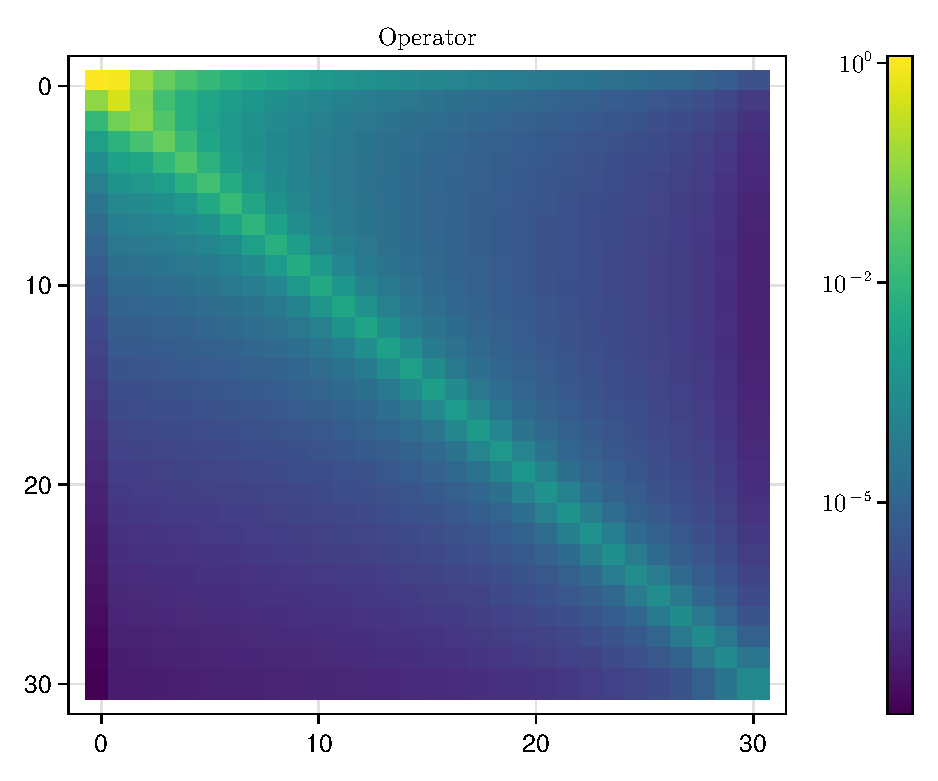
\includegraphics[width=0.5\linewidth]{results/morse/full-operator.pdf}
  \caption[Full Morse operator]{The full operator constructed from the $G=8$th order monomial expansion $K_G$ of the morse potential function $K_{C_a, l_a, C_r, l_r}(r)$ with parameters as given above.}
  \label{fig:morse-operator}
\end{figure}

\begin{figure}[H]
  \centering
  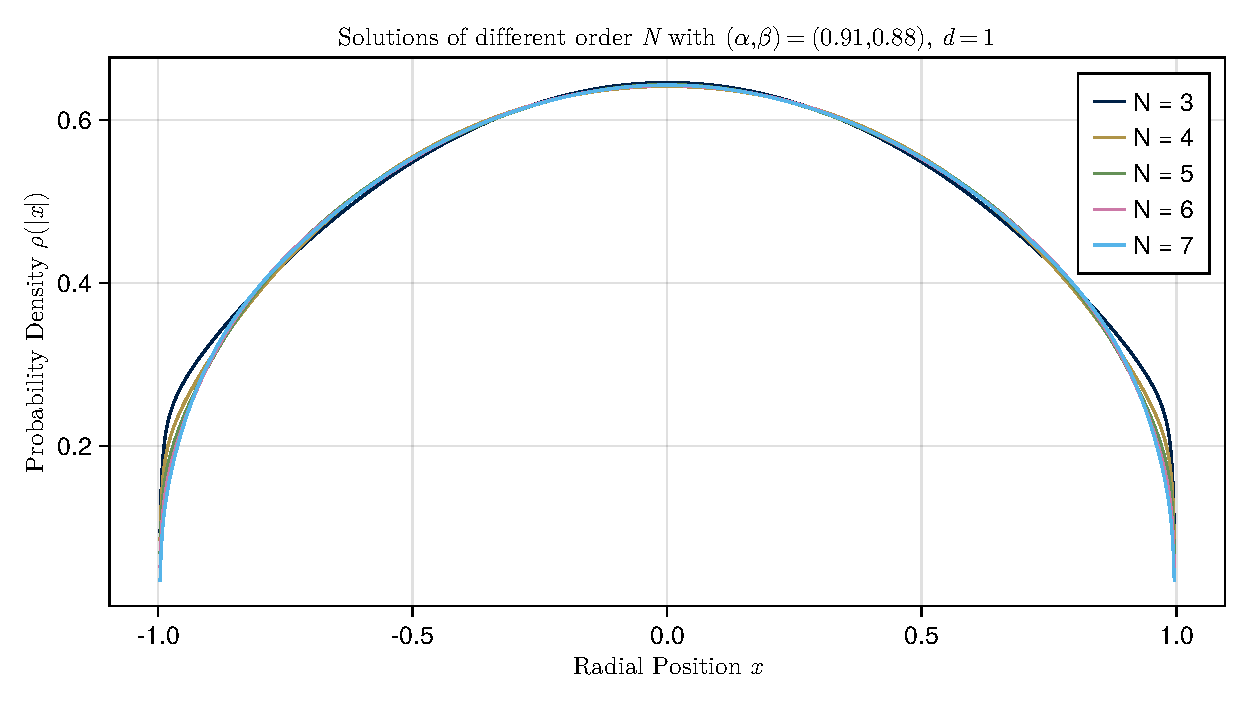
\includegraphics[width=0.8\linewidth]{results/morse/solution-increasing-order.pdf}
  \caption[General kernel solutions of increasing order]{Solutions $\rho_N(x)$ of increasing order $N$ in the general kernel setting with a monomial expansion of highest order $G = 8$ of the morse potential $K_{C_a, l_a, C_r, l_r}(r)$.}
  \label{fig:morse-solution-increasing-order}
\end{figure}

\begin{figure}[H]
  \centering
  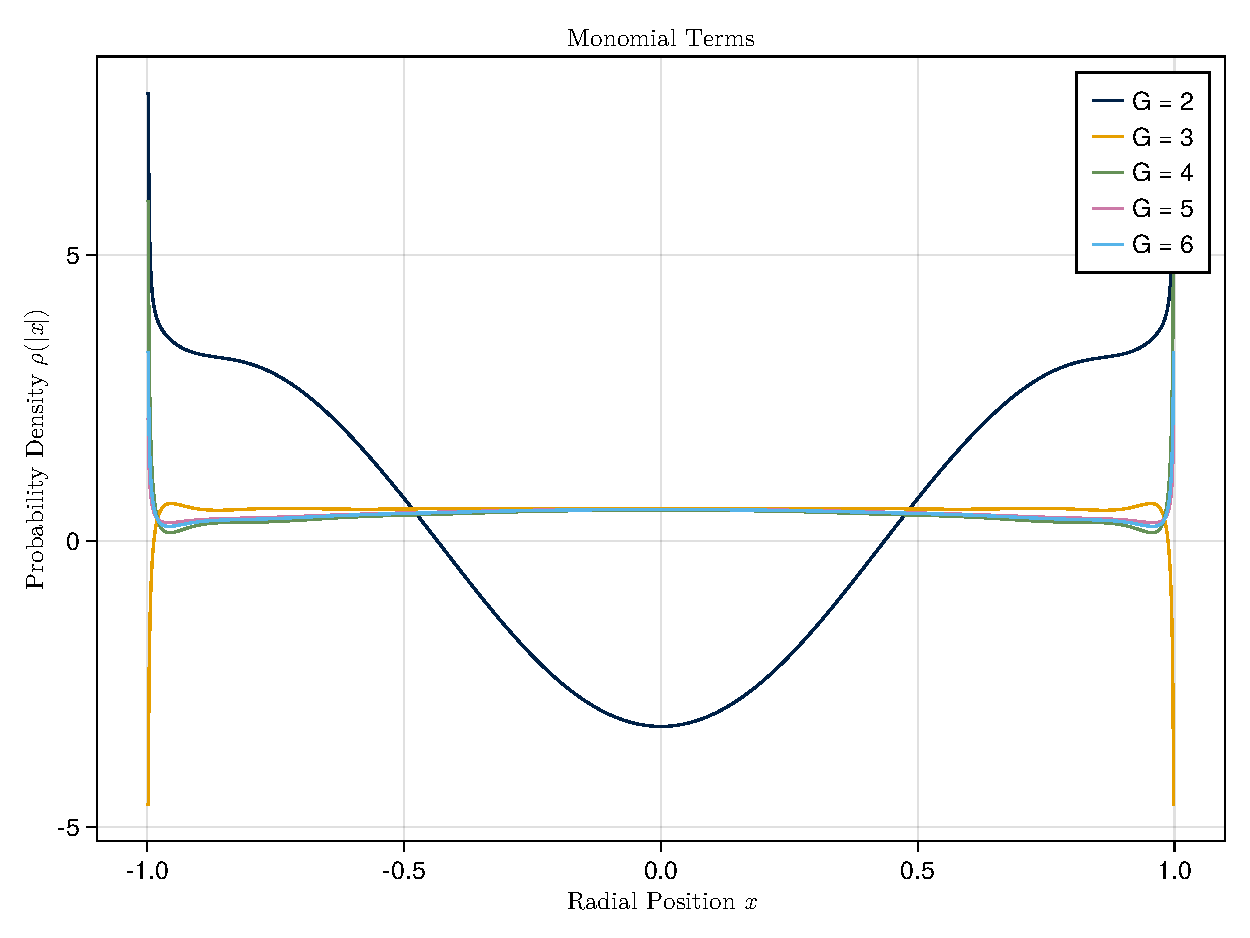
\includegraphics[width=0.7\linewidth]{results/morse/monomial-solutions.pdf}
  \caption[]{Solutions $\rho_8(x)$ for an increasing number of terms $G$ in the monomial expansion of a general kernel $K$, in this case given by the morse potential $K_{C_a, l_a, C_r, l_r}(r)$. So each solution $\rho_8(x)$ is the sum of $8$ Jacobi polynomials weighted by the solution coefficients.}
  \label{fig:monomial-solutions}
\end{figure}

As one can see, the solutions improve the better the approximation of the general kernel $K$ becomes with growing order $G$ of its monomial expansion.
To make a better statement about this numerical behaviour, consider \Cref{fig:monomial-basis-convergence}.

\begin{figure}[H]
  \centering
  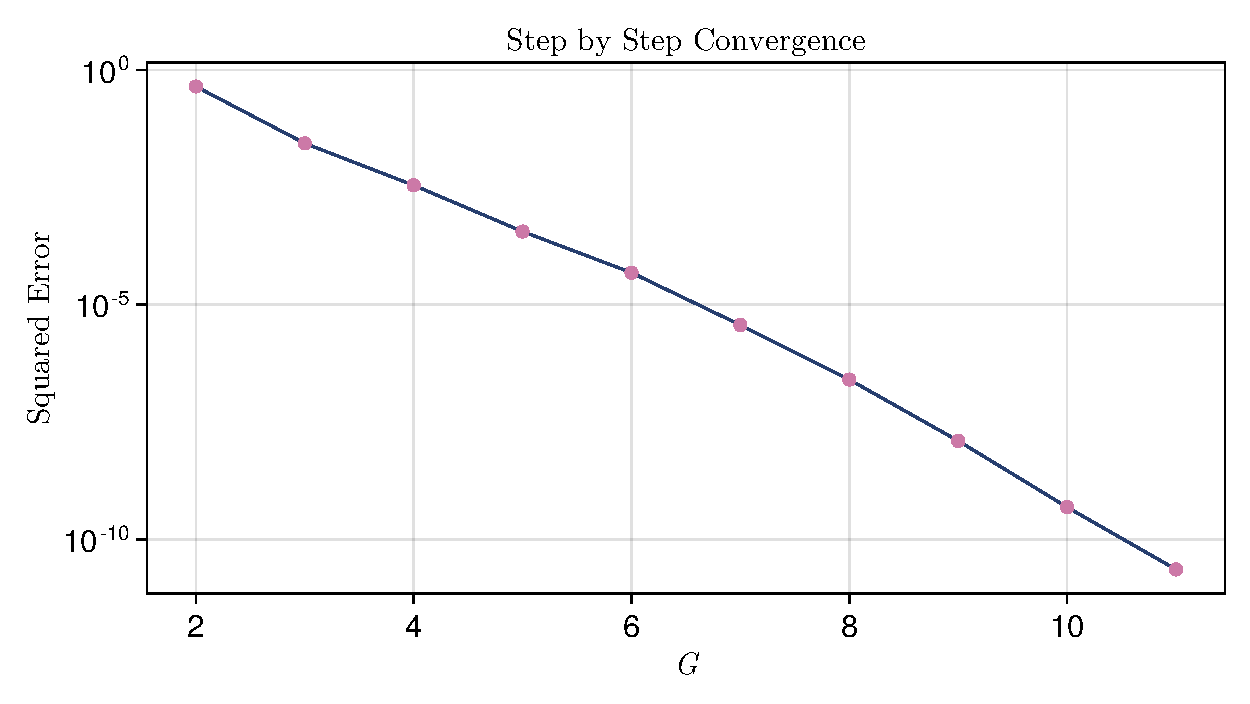
\includegraphics[width=0.7\linewidth]{results/morse/monomial-basis-convergence.pdf}
  \caption[Step-by-step convergence of solutions when increasing the degree of the monomial]{
    Convergence of numerical solutions $\rho_N(x)$ as compared to $\rho_{24}(x)$, visualised using the squared error of the pointwise evaluation of both functions in $200$ points.
    The solver again uses $K(r) = K_{C_a, l_a, C_r, l_r}(r)$.
  }
  \label{fig:monomial-basis-convergence}
\end{figure}

\begin{figure}[H]
  \centering
  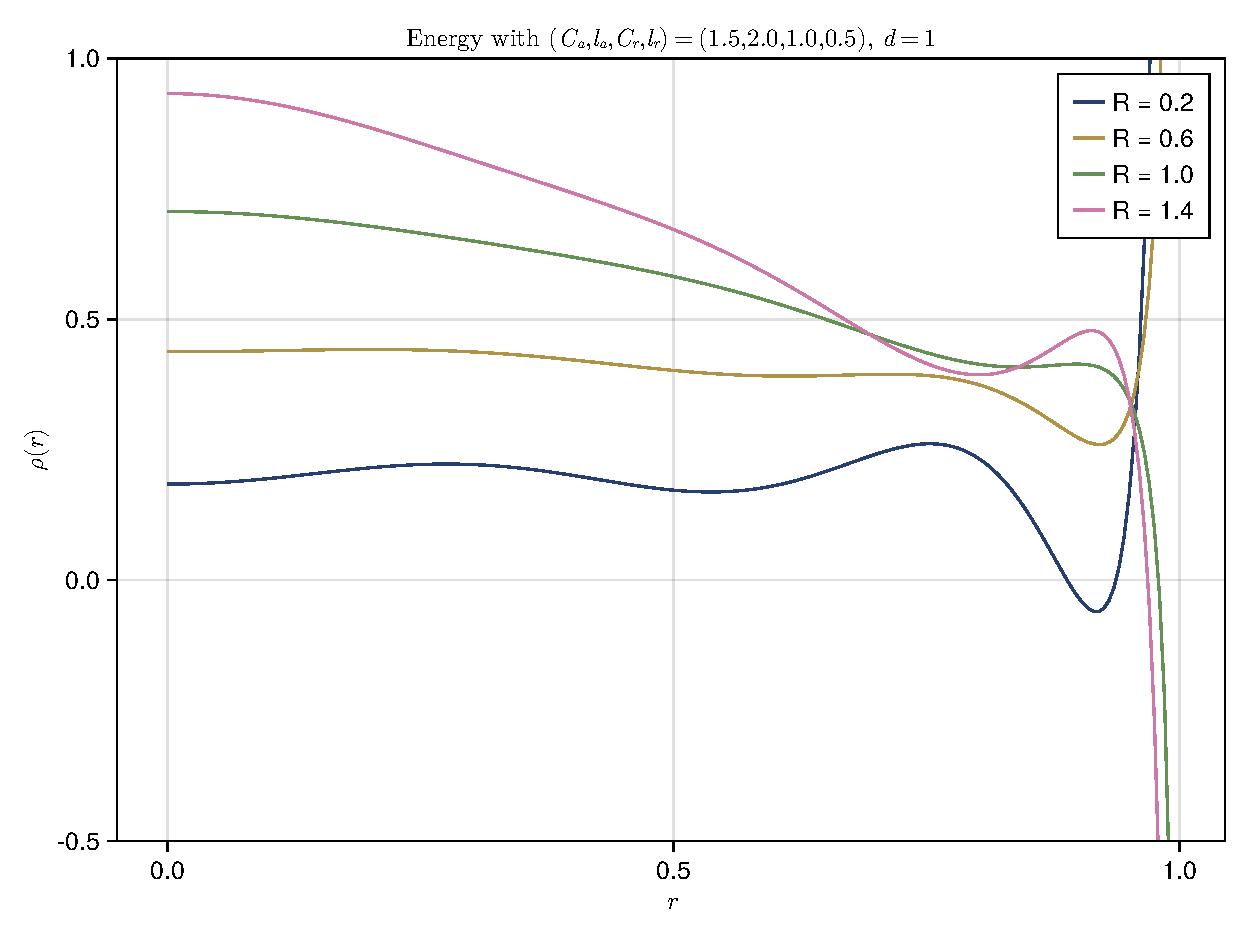
\includegraphics[width=0.7\linewidth]{results/morse/varying-R-solutions.pdf}
  \caption[Solutions with varying $R$]{General kernel solutions ($N = 6$, $G = 8$) with varying $R$ when using the Morse potential $K_{C_a, l_a, C_r, l_r}(r)$ with parameters as given above.}
  \label{fig:varying-R-solutions}
\end{figure}

% There is strong numerical evidence for ... (a ``conjecture'').
% This is a current topic of discussion in the numerical analysis community.
